\documentclass[11pt,aspectratio=43]{beamer}

\usepackage{amsmath,amssymb}
\usepackage{booktabs}
\usepackage{graphicx}
\usepackage{xcolor}
\usepackage{tikz}
\usetikzlibrary{arrows.meta,positioning,shapes.geometric,calc,decorations.pathreplacing}

\graphicspath{{./}{../overview/v4/slides/}{../overview/v1/figs/}}

\definecolor{accent}{HTML}{2E75B6}
\definecolor{red2}{HTML}{C0392B}
\definecolor{green2}{HTML}{27AE60}
\definecolor{orange2}{HTML}{E67E22}
\definecolor{gray2}{HTML}{7F8C8D}

\setbeameroption{hide notes}
\setbeamertemplate{navigation symbols}{}
\setbeamersize{text margin left=0.9cm,text margin right=0.9cm}

\setbeamercolor{normal text}{fg=black,bg=white}
\setbeamercolor{frametitle}{fg=black,bg=white}
\setbeamercolor{title}{fg=black}
\setbeamercolor{structure}{fg=black}
\setbeamercolor{alerted text}{fg=accent}
\setbeamercolor{block title}{fg=black,bg=black!10}
\setbeamercolor{block body}{fg=black,bg=black!3}
\setbeamercolor{itemize item}{fg=black}
\setbeamercolor{itemize subitem}{fg=black}

\setbeamerfont{title}{size=\normalsize,series=\bfseries}
\setbeamerfont{frametitle}{size=\normalsize,series=\bfseries}
\setbeamerfont{block title}{size=\small,series=\bfseries}
\setbeamerfont{block body}{size=\small}

\setbeamertemplate{footline}{%
  \leavevmode%
  \hbox{%
    \begin{beamercolorbox}[wd=\paperwidth,ht=2.5ex,dp=1.0ex,rightskip=0.9cm]{author in head/foot}%
      \hfill\insertframenumber
    \end{beamercolorbox}%
  }%
}

\title{RL for CXL Memory Pooling:\\When Learning Helps, When Greedy Wins}
\author{Pulak Mehrotra}
\date{May 2026}

\begin{document}

\begin{frame}[plain]
  \titlepage
\end{frame}

% =========================================================================
% MAIN SLIDE 1 -- Why RL
% =========================================================================

\begin{frame}[shrink=7]{Why RL was worth trying: greedy is local, the objective is global.}

  \begin{columns}[T,onlytextwidth]

    \column{0.48\textwidth}
      \vspace{0.2em}
      \begin{block}{Systems problem}
        \small
        Each VM arrives online and must be placed on one reachable CXL Memory
        Pool Device (MPD).  The action is local, but the cost is the
        \textbf{peak MPD load over the full trace}.
      \end{block}

      \vspace{0.5em}
      \begin{itemize}
        \setlength{\itemsep}{0.40em}
        \item \textbf{Greedy:} pick the least-loaded reachable MPD now.
        \item \textbf{Failure mode:} filling a shared MPD can remove headroom
              for a different host later.
        \item \textbf{RL hypothesis:} learn when current load is transient
              versus sticky from trace replay.
      \end{itemize}

    \column{0.52\textwidth}
      \begin{center}
      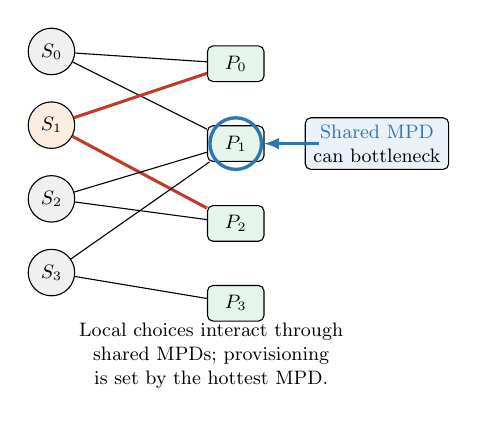
\begin{tikzpicture}[
          scale=0.78,
          transform shape,
          every node/.style={font=\small},
          host/.style={draw,circle,fill=black!6,minimum size=0.72cm},
          mpd/.style={draw,rounded corners=2pt,fill=green2!12,
                      minimum width=0.92cm,minimum height=0.58cm},
          callout/.style={draw,rounded corners=2pt,fill=accent!10,
                          text width=2.1cm,align=center,minimum height=0.7cm},
      ]
        \node[host] (h0) at (0,2.2) {$S_0$};
        \node[host,fill=orange2!14] (h1) at (0,1.0) {$S_1$};
        \node[host] (h2) at (0,-0.2) {$S_2$};
        \node[host] (h3) at (0,-1.4) {$S_3$};

        \node[mpd] (p0) at (3.0,2.0) {$P_0$};
        \node[mpd] (p1) at (3.0,0.7) {$P_1$};
        \node[mpd] (p2) at (3.0,-0.6) {$P_2$};
        \node[mpd] (p3) at (3.0,-1.9) {$P_3$};

        \draw (h0) -- (p0);
        \draw (h0) -- (p1);
        \draw[red2,line width=1.1pt] (h1) -- (p0);
        \draw[red2,line width=1.1pt] (h1) -- (p2);
        \draw (h2) -- (p1);
        \draw (h2) -- (p2);
        \draw (h3) -- (p1);
        \draw (h3) -- (p3);

        \draw[accent,line width=1.2pt] ($(p1)+(-0.42,0)$) arc (180:540:0.42);
        \node[callout] at (5.3,0.7) {\textcolor{accent}{Shared MPD}\\can bottleneck};
        \draw[-{Latex[length=2mm]},accent,line width=1.1pt] (4.35,0.7) -- (3.45,0.7);

        \node[align=center,text width=5.2cm] at (2.6,-2.75)
          {Local choices interact through shared MPDs; provisioning is set by the hottest MPD.};
      \end{tikzpicture}
      \end{center}

  \end{columns}

\end{frame}

% =========================================================================
% MAIN SLIDE 2 -- Greedy / optimal / RL
% =========================================================================

\begin{frame}[shrink=8]{Greedy is deployable; optimal is a benchmark; RL tries to close the gap.}

  \begin{columns}[T,onlytextwidth]

    \column{0.46\textwidth}
      \vspace{0.25em}
      \resizebox{\linewidth}{!}{%
      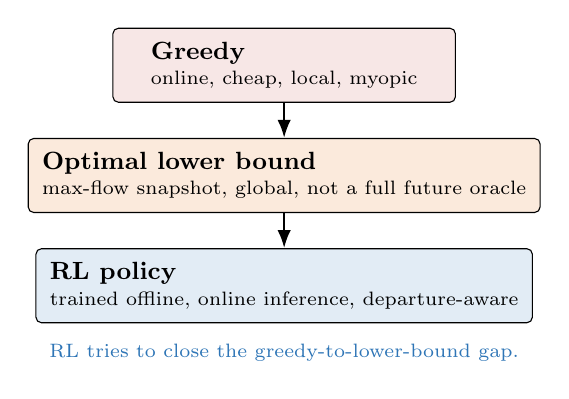
\begin{tikzpicture}[
          every node/.style={font=\small},
          box/.style={draw,rounded corners=2pt,minimum width=4.35cm,
                      minimum height=0.85cm,align=left,inner sep=5pt},
          arr/.style={-{Latex[length=2.3mm]},line width=0.9pt},
      ]
        \node[box,fill=red2!12] (g) at (0,3.2)
          {\textbf{Greedy}\\[-0.2em]
           \scriptsize online, cheap, local, myopic};
        \node[box,fill=orange2!16] (o) at (0,1.8)
          {\textbf{Optimal lower bound}\\[-0.2em]
           \scriptsize max-flow snapshot, global, not a full future oracle};
        \node[box,fill=accent!14] (r) at (0,0.4)
          {\textbf{RL policy}\\[-0.2em]
           \scriptsize trained offline, online inference, departure-aware};

        \draw[arr] (g) -- (o);
        \draw[arr] (o) -- (r);
        \node[align=center,text=accent,font=\scriptsize] at (0,-0.45)
          {RL tries to close the greedy-to-lower-bound gap.};
      \end{tikzpicture}
      }

    \column{0.54\textwidth}
      \vspace{0.05em}
      \begin{itemize}
        \setlength{\itemsep}{0.38em}
        \item Greedy is the right baseline because it can run at every VM arrival.
        \item The exact solver computes a tight per-snapshot lower bound
              $t^*(s)$ using Dinic max-flow.
        \item The lower bound is diagnostic: it shows whether the current
              state wasted peak capacity.
        \item RL is only worth considering if trace structure creates a
              repeatable policy better than local load balancing.
      \end{itemize}

      \vspace{0.2em}
      \small\textit{Careful claim: ``optimal'' is a lower bound and shaping
      signal, not a deployable 14-day oracle.}

  \end{columns}

\end{frame}

% =========================================================================
% MAIN SLIDE 3 -- Latest result
% =========================================================================

\begin{frame}[shrink=5]{Best result: RL helps on churn-heavy traces, but generalization is not solved.}

  \begin{columns}[T,onlytextwidth]

    \column{0.58\textwidth}
      \vspace{0.2em}
      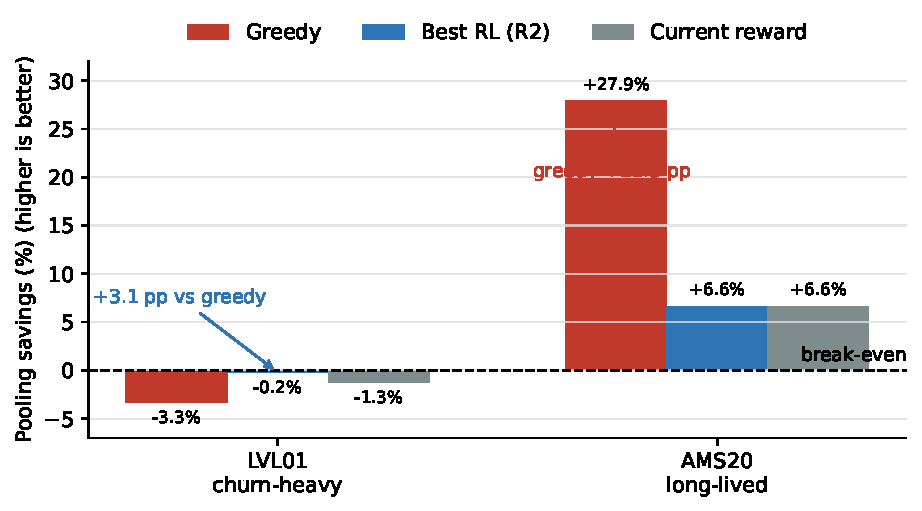
\includegraphics[width=\linewidth]{rl_vs_greedy_latest.pdf}

    \column{0.42\textwidth}
      \vspace{0.35em}
      \begin{itemize}
        \setlength{\itemsep}{0.65em}
        \item \textbf{LVL01:} best RL (R2) reaches \textbf{$-0.2\%$}
              savings vs. greedy \textbf{$-3.3\%$}.
        \item This is a \textbf{+3.1 percentage point} improvement,
              nearly break-even.
        \item \textbf{AMS20:} greedy wins decisively: \textbf{$+27.9\%$}
              savings vs. RL variants around \textbf{$+6.6\%$}.
        \item This is a workload-regime split, not a universal RL win.
      \end{itemize}

  \end{columns}

\end{frame}

\begin{frame}[shrink=5]{The policy generalized to the lifetime regime it mostly saw.}

  \begin{columns}[T,onlytextwidth]

    \column{0.64\textwidth}
      \vspace{0.15em}
      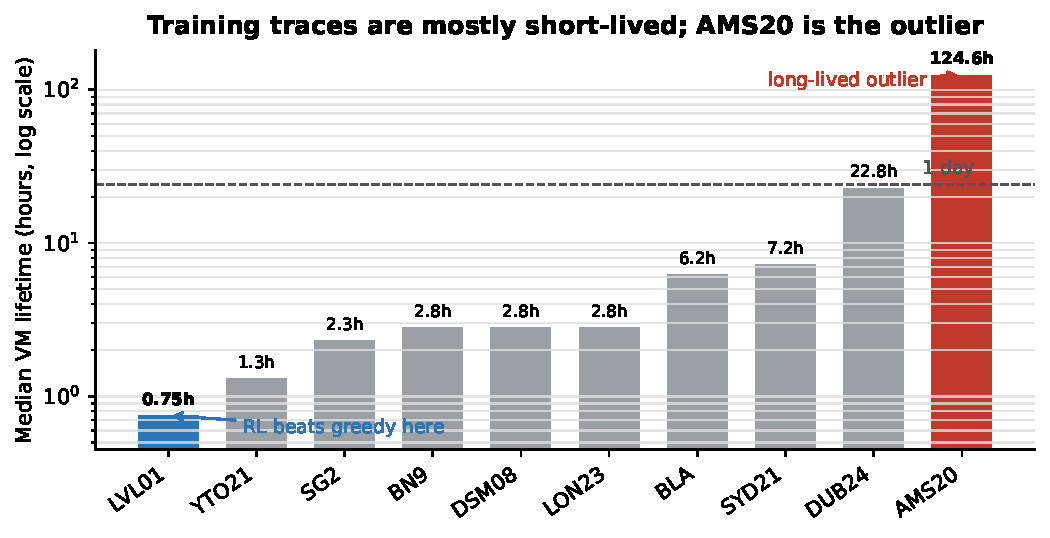
\includegraphics[width=\linewidth]{trace_lifetime_similarity.pdf}

    \column{0.36\textwidth}
      \vspace{0.3em}
      \begin{itemize}
        \setlength{\itemsep}{0.7em}
        \item The multi-trace training pool is mostly short-lived; most median
              lifetimes are under a day.
        \item \textbf{LVL01} is the churn-heavy regime where RL beat greedy:
              median \textbf{0.75h}, \textbf{56.7\%} of VMs $<1$h.
        \item \textbf{AMS20} is the long-lived outlier:
              median \textbf{124.6h}, \textbf{49.3\%} of VMs $>7$d.
        \item So the failure is distribution shift: the policy learned
              churn-oriented placement behavior.
      \end{itemize}

  \end{columns}

\end{frame}

% =========================================================================
% MAIN SLIDE 4 -- Sticky load
% =========================================================================

\begin{frame}[shrink=6]{Sticky load explains why lifetime regime changes the best policy.}

  \begin{columns}[T,onlytextwidth]

    \column{0.43\textwidth}
      \vspace{0.15em}
      \begin{itemize}
        \setlength{\itemsep}{0.55em}
        \item \textbf{Transient load:} short-lived VMs drain soon, so a full MPD
              can become useful again.
        \item \textbf{Sticky load:} long-lived VMs stay resident, so today's
              imbalance becomes tomorrow's bottleneck.
        \item Greedy is strong when load is sticky: the least-loaded reachable
              MPD is often the right local choice.
        % \item RL has more room when load is transient: departure timing can make
              a currently-full MPD the better future choice.
      \end{itemize}

      \vspace{0.25em}
      \scriptsize\textit{This is why the same policy can help on LVL01 but fail
      to generalize to AMS20.}

    \column{0.57\textwidth}
      \begin{center}
      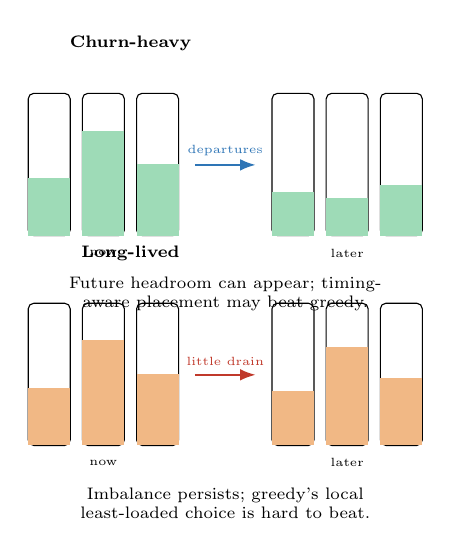
\begin{tikzpicture}[
          scale=0.86,
          transform shape,
          every node/.style={font=\scriptsize},
          mpd/.style={draw,rounded corners=2pt,minimum width=0.62cm,
                      minimum height=2.1cm,anchor=south},
          load/.style={draw=none,anchor=south,minimum width=0.62cm},
          arr/.style={-{Latex[length=2.0mm]},line width=0.8pt},
      ]
        \node[font=\scriptsize\bfseries] at (1.2,2.85) {Churn-heavy};
        \node[mpd] (c0) at (0.0,0) {};
        \node[mpd] (c1) at (0.8,0) {};
        \node[mpd] (c2) at (1.6,0) {};
        \node[load,fill=green2!45,minimum height=0.85cm] at (0.0,0) {};
        \node[load,fill=green2!45,minimum height=1.55cm] at (0.8,0) {};
        \node[load,fill=green2!45,minimum height=1.05cm] at (1.6,0) {};
        \node[font=\tiny] at (0.8,-0.25) {now};

        \draw[arr,accent] (2.15,1.05) -- (3.05,1.05)
          node[midway,above,font=\tiny] {departures};

        \node[mpd] (c3) at (3.6,0) {};
        \node[mpd] (c4) at (4.4,0) {};
        \node[mpd] (c5) at (5.2,0) {};
        \node[load,fill=green2!45,minimum height=0.65cm] at (3.6,0) {};
        \node[load,fill=green2!45,minimum height=0.55cm] at (4.4,0) {};
        \node[load,fill=green2!45,minimum height=0.75cm] at (5.2,0) {};
        \node[font=\tiny] at (4.4,-0.25) {later};
        \node[align=center,text width=5.0cm] at (2.6,-0.85)
          {Future headroom can appear; timing-aware placement may beat greedy.};

        \begin{scope}[yshift=-3.1cm]
          \node[font=\scriptsize\bfseries] at (1.2,2.85) {Long-lived};
          \node[mpd] at (0.0,0) {};
          \node[mpd] at (0.8,0) {};
          \node[mpd] at (1.6,0) {};
          \node[load,fill=orange2!55,minimum height=0.85cm] at (0.0,0) {};
          \node[load,fill=orange2!55,minimum height=1.55cm] at (0.8,0) {};
          \node[load,fill=orange2!55,minimum height=1.05cm] at (1.6,0) {};
          \node[font=\tiny] at (0.8,-0.25) {now};

          \draw[arr,red2] (2.15,1.05) -- (3.05,1.05)
            node[midway,above,font=\tiny] {little drain};

          \node[mpd] at (3.6,0) {};
          \node[mpd] at (4.4,0) {};
          \node[mpd] at (5.2,0) {};
          \node[load,fill=orange2!55,minimum height=0.80cm] at (3.6,0) {};
          \node[load,fill=orange2!55,minimum height=1.45cm] at (4.4,0) {};
          \node[load,fill=orange2!55,minimum height=1.00cm] at (5.2,0) {};
          \node[font=\tiny] at (4.4,-0.25) {later};
          \node[align=center,text width=5.0cm] at (2.6,-0.85)
            {Imbalance persists; greedy's local least-loaded choice is hard to beat.};
        \end{scope}
      \end{tikzpicture}
      \end{center}

  \end{columns}

\end{frame}

% =========================================================================
% MAIN SLIDE 5 -- SAC
% =========================================================================

\begin{frame}[shrink=7]{SAC was chosen because collapse was the first failure mode.}

  \begin{columns}[T,onlytextwidth]

    \column{0.48\textwidth}
      \vspace{0.1em}
      \begin{itemize}
        \setlength{\itemsep}{0.45em}
        \item Early policies collapsed to one or two MPDs even when load changed.
        \item SAC adds an entropy term, keeping the policy from becoming
              deterministic too early.
        \item Off-policy replay fits trace replay: one allocation experience can
              support many gradient updates.
        \item SB3 SAC worked cleanly with 32 parallel environments, which made
              controlled ablations practical.
      \end{itemize}

      \vspace{0.25em}
      \small\textit{I avoid PPO-specific claims here; the documented comparison
      is against LCPO and A2C.}

    \column{0.52\textwidth}
      \begin{center}
      \resizebox{0.95\linewidth}{!}{%
      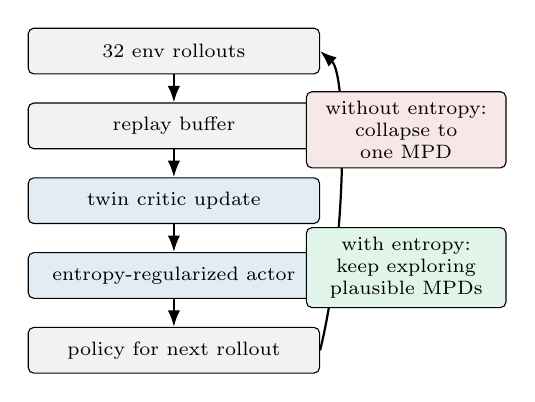
\begin{tikzpicture}[
          every node/.style={font=\scriptsize},
          box/.style={draw,rounded corners=2pt,fill=black!5,
                      minimum width=3.7cm,minimum height=0.58cm,
                      align=center,inner sep=4pt},
          acbox/.style={draw,rounded corners=2pt,fill=accent!14,
                        minimum width=3.7cm,minimum height=0.58cm,
                        align=center,inner sep=4pt},
          arr/.style={-{Latex[length=2.1mm]},line width=0.8pt},
      ]
        \node[box] (env) at (0,3.2) {32 env rollouts};
        \node[box] (buf) at (0,2.25) {replay buffer};
        \node[acbox] (critic) at (0,1.30) {twin critic update};
        \node[acbox] (actor) at (0,0.35) {entropy-regularized actor};
        \node[box] (pol) at (0,-0.60) {policy for next rollout};
        \draw[arr] (env) -- (buf);
        \draw[arr] (buf) -- (critic);
        \draw[arr] (critic) -- (actor);
        \draw[arr] (actor) -- (pol);
        \draw[arr] (pol.east) .. controls (2.2,0.8) and (2.2,2.9) .. (env.east);

        \node[draw,rounded corners=2pt,fill=red2!12,align=center,text width=2.3cm]
          at (2.95,2.2) {without entropy:\\collapse to one MPD};
        \node[draw,rounded corners=2pt,fill=green2!14,align=center,text width=2.3cm]
          at (2.95,0.45) {with entropy:\\keep exploring plausible MPDs};
      \end{tikzpicture}
      }
      \end{center}

  \end{columns}

\end{frame}

% =========================================================================
% MAIN SLIDE 5 -- Augmentation knobs
% =========================================================================

\begin{frame}[shrink=5]{Augmentation was domain randomization, not random noise.}

  \begin{columns}[T,onlytextwidth]

    \column{0.50\textwidth}
      \vspace{0.2em}
      \begin{itemize}
        \setlength{\itemsep}{0.65em}
        \item VM memory sizes are SKU-like; per-VM scaling creates fake VM types.
        \item So randomization happens at the \textbf{episode} level.
        \item Enabled knobs: trace ID, pod seed, episode memory scale.
        \item Disabled until validated: arrival jitter, lifetime perturbation,
              link failures.
      \end{itemize}

      \vspace{0.4em}
      \begin{block}{Scale range}
        \small
        Use $s \sim \mathrm{Tri}(0.7, 1.0, 1.2)$: enough load diversity,
        without making HOTFIX dropout dominate the episode.
      \end{block}

    \column{0.50\textwidth}
      \begin{center}
      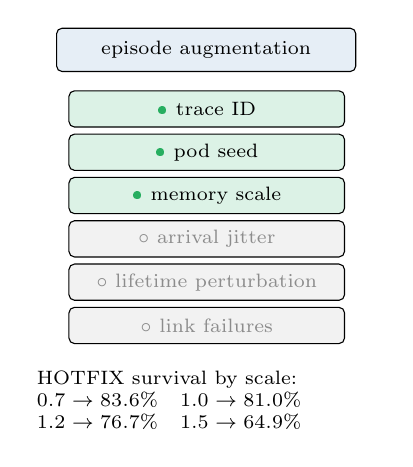
\begin{tikzpicture}[
          every node/.style={font=\scriptsize},
          knobon/.style={draw,rounded corners=2pt,fill=green2!16,
                         minimum width=3.5cm,minimum height=0.46cm,align=left,inner sep=3pt},
          knoboff/.style={draw,rounded corners=2pt,fill=black!5,text=black!45,
                          minimum width=3.5cm,minimum height=0.46cm,align=left,inner sep=3pt},
      ]
        \node[draw,rounded corners=2pt,fill=accent!12,minimum width=3.8cm,
              minimum height=0.55cm,align=center] at (0,3.5) {episode augmentation};
        \node[knobon,anchor=west] at (-1.75,2.75) {\textcolor{green2}{\textbullet}\ trace ID};
        \node[knobon,anchor=west] at (-1.75,2.20) {\textcolor{green2}{\textbullet}\ pod seed};
        \node[knobon,anchor=west] at (-1.75,1.65) {\textcolor{green2}{\textbullet}\ memory scale};
        \node[knoboff,anchor=west] at (-1.75,1.10) {$\circ$ arrival jitter};
        \node[knoboff,anchor=west] at (-1.75,0.55) {$\circ$ lifetime perturbation};
        \node[knoboff,anchor=west] at (-1.75,0.00) {$\circ$ link failures};

        \node[align=left,text width=4.3cm] at (0,-0.95)
          {HOTFIX survival by scale:\\
           $0.7 \rightarrow 83.6\%$\quad
           $1.0 \rightarrow 81.0\%$\\
           $1.2 \rightarrow 76.7\%$\quad
           $1.5 \rightarrow 64.9\%$};
      \end{tikzpicture}
      \end{center}

  \end{columns}

\end{frame}

% =========================================================================
% MAIN SLIDE 6 -- Augmentation helped?
% =========================================================================

\begin{frame}[shrink=5]{Augmentation improved robustness, but not lifetime-distribution shift.}

  \begin{columns}[T,onlytextwidth]

    \column{0.50\textwidth}
      \vspace{0.2em}
      \begin{itemize}
        \setlength{\itemsep}{0.65em}
        \item Single-trace training overfit and was brittle on unseen traces.
        \item Multi-trace + pod seed + scale augmentation made stable held-out
              evaluation possible.
        \item Training savings improved from run7's $\sim$\textbf{1.3\%}
              plateau to $\sim$\textbf{5\%} in later multi-trace ablations.
        \item That comparison is confounded by \texttt{skip-hotfix}, so the
              strongest claim is robustness, not a clean causal win.
      \end{itemize}

    \column{0.50\textwidth}
      \begin{center}
      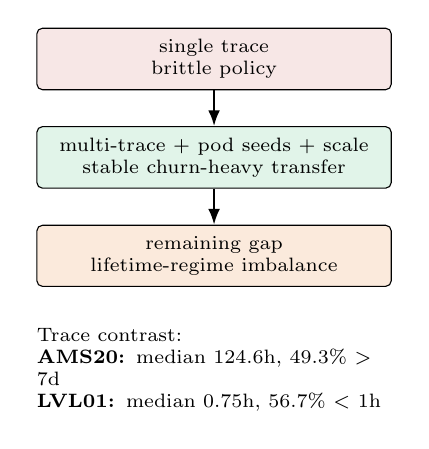
\begin{tikzpicture}[
          every node/.style={font=\scriptsize},
          box/.style={draw,rounded corners=2pt,fill=black!5,
                      minimum width=4.5cm,minimum height=0.72cm,align=center,inner sep=4pt},
          arr/.style={-{Latex[length=2.0mm]},line width=0.8pt},
      ]
        \node[box,fill=red2!12] (single) at (0,3.1)
          {single trace\\brittle policy};
        \node[box,fill=green2!14] (aug) at (0,1.85)
          {multi-trace + pod seeds + scale\\stable churn-heavy transfer};
        \node[box,fill=orange2!16] (gap) at (0,0.60)
          {remaining gap\\lifetime-regime imbalance};
        \draw[arr] (single) -- (aug);
        \draw[arr] (aug) -- (gap);

        \node[align=left,text width=4.5cm] at (0,-0.85)
          {Trace contrast:\\
           \textbf{AMS20:} median 124.6h, 49.3\% $>$ 7d\\
           \textbf{LVL01:} median 0.75h, 56.7\% $<$ 1h};
      \end{tikzpicture}
      \end{center}

  \end{columns}

\end{frame}

% =========================================================================
% MAIN SLIDE 7 -- Proxy versus terminal reward
% =========================================================================

\begin{frame}[shrink=6]{Proxy rewards teach every placement; terminal reward grades the whole trace.}

  \begin{columns}[T,onlytextwidth]

    \column{0.46\textwidth}
      \vspace{0.15em}
      \begin{block}{Proxy reward}
        \small
        A local signal after each VM placement: did this action reduce
        immediate pressure, imbalance, or an estimated optimality gap?
      \end{block}

      \vspace{0.45em}
      \begin{block}{Terminal reward}
        \small
        The actual objective after replaying the trace:
        \[
          \frac{\text{greedy peak} - \text{policy peak}}{\text{greedy peak}}.
        \]
      \end{block}

      \vspace{0.35em}
      \scriptsize\textit{Design tension: dense feedback is learnable but can
      be misaligned; exact feedback is aligned but arrives too late for easy
      credit assignment.}

    \column{0.54\textwidth}
      \begin{center}
      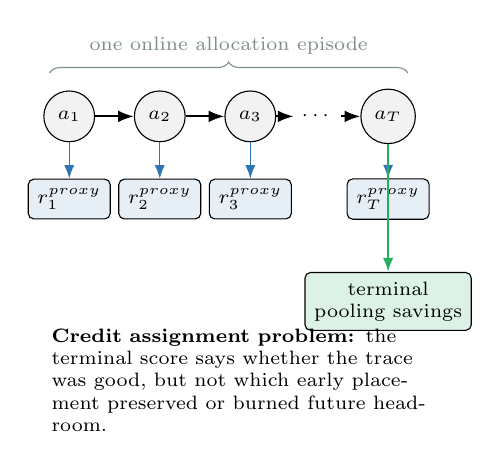
\begin{tikzpicture}[
          every node/.style={font=\scriptsize},
          actionstep/.style={draw,circle,fill=black!5,minimum size=0.58cm},
          proxy/.style={draw,rounded corners=2pt,fill=accent!12,
                        align=center,minimum width=0.95cm,minimum height=0.45cm},
          terminal/.style={draw,rounded corners=2pt,fill=green2!16,
                           align=center,minimum width=1.55cm,minimum height=0.55cm},
          arr/.style={-{Latex[length=2.0mm]},line width=0.8pt},
      ]
        \node[actionstep] (a1) at (0,1.8) {$a_1$};
        \node[actionstep] (a2) at (1.15,1.8) {$a_2$};
        \node[actionstep] (a3) at (2.30,1.8) {$a_3$};
        \node at (3.15,1.8) {$\cdots$};
        \node[actionstep] (at) at (4.05,1.8) {$a_T$};

        \draw[arr] (a1) -- (a2);
        \draw[arr] (a2) -- (a3);
        \draw[arr] (a3) -- (2.85,1.8);
        \draw[arr] (3.45,1.8) -- (at);

        \node[proxy] (r1) at (0,0.75) {$r_1^{proxy}$};
        \node[proxy] (r2) at (1.15,0.75) {$r_2^{proxy}$};
        \node[proxy] (r3) at (2.30,0.75) {$r_3^{proxy}$};
        \node[proxy] (rt) at (4.05,0.75) {$r_T^{proxy}$};

        \draw[-{Latex[length=1.7mm]},accent] (a1) -- (r1);
        \draw[-{Latex[length=1.7mm]},accent] (a2) -- (r2);
        \draw[-{Latex[length=1.7mm]},accent] (a3) -- (r3);
        \draw[-{Latex[length=1.7mm]},accent] (at) -- (rt);

        \node[terminal] (term) at (4.05,-0.55)
          {terminal\\pooling savings};
        \draw[-{Latex[length=1.8mm]},green2,line width=0.9pt] (at) -- (term);

        \draw[decorate,decoration={brace,amplitude=4pt},gray2]
          (-0.25,2.35) -- (4.30,2.35)
          node[midway,yshift=0.35cm,align=center]
          {one online allocation episode};

        \node[align=left,text width=4.85cm] at (2.20,-1.55)
          {\textbf{Credit assignment problem:} the terminal score says whether
           the trace was good, but not which early placement preserved or burned
           future headroom.};
      \end{tikzpicture}
      \end{center}

  \end{columns}

\end{frame}

% =========================================================================
% MAIN SLIDE 8 -- Reward design
% =========================================================================

\begin{frame}[shrink=8]{Reward design aligns local decisions with the global peak objective.}

  \begin{columns}[T,onlytextwidth]

    \column{0.42\textwidth}
      \vspace{0.05em}
      \begin{itemize}
        \setlength{\itemsep}{0.26em}
        \item \textbf{Proxy rewards:} dense and learnable, but can optimize
              the wrong thing.
        \item \textbf{Terminal reward:} exactly pooling savings, but sparse
              over thousands of decisions.
        \item \textbf{Optimal gap:} max-flow lower bound; principled but
              expensive.
        % \item \textbf{Held-out result:} no reward dominates; R1--R3/current
              % trail greedy, while R4--R5 improve over greedy on LVL01.
        \item \textbf{Takeaway:} reward design changes the workload regime where
              RL helps, not just the training curve.
      \end{itemize}

      \vspace{0.15em}
      \scriptsize\textit{Measurement problem: which scalar signal faithfully
      reflects the peak-memory objective at each local decision?}

    \column{0.58\textwidth}
      \vspace{0.1em}
      \begin{center}
        \textbf{\scriptsize All reward ablations compared to greedy.}

        \vspace{0.25em}
        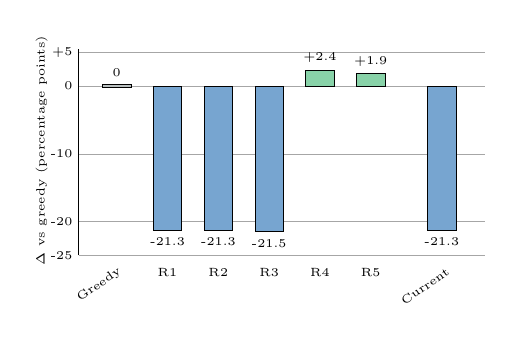
\begin{tikzpicture}[
            scale=0.86,
            transform shape,
            every node/.style={font=\scriptsize},
            rlbar/.style={fill=accent!65,draw=black,line width=0.25pt},
            rlpos/.style={fill=green2!55,draw=black,line width=0.25pt},
            greedybar/.style={fill=gray2!55,draw=black,line width=0.25pt},
            axis/.style={black,line width=0.4pt},
        ]
          % Delta-vs-greedy chart: y = (delta_pp + 25) * 0.10.
          \draw[axis] (-0.35,2.50) -- (5.65,2.50);
          \draw[axis] (-0.35,0) -- (-0.35,3.05);
          \foreach \y/\lab in {0/-25,0.5/-20,1.5/-10,2.5/0,3.0/+5} {
            \draw[black!35,line width=0.25pt] (-0.35,\y) -- (5.65,\y);
            \node[anchor=east,font=\tiny] at (-0.32,\y) {\lab};
          }
          \draw[greedybar] (0.00,2.48) rectangle (0.42,2.52);
          \draw[rlbar]     (0.75,2.50) rectangle (1.17,0.37);
          \draw[rlbar]     (1.50,2.50) rectangle (1.92,0.37);
          \draw[rlbar]     (2.25,2.50) rectangle (2.67,0.35);
          \draw[rlpos]     (3.00,2.50) rectangle (3.42,2.74);
          \draw[rlpos]     (3.75,2.50) rectangle (4.17,2.69);
          \draw[rlbar]     (4.80,2.50) rectangle (5.22,0.37);

          \node[font=\tiny,rotate=35,anchor=east] at (0.36,-0.15) {Greedy};
          \node[font=\tiny] at (0.96,-0.25) {R1};
          \node[font=\tiny] at (1.71,-0.25) {R2};
          \node[font=\tiny] at (2.46,-0.25) {R3};
          \node[font=\tiny] at (3.21,-0.25) {R4};
          \node[font=\tiny] at (3.96,-0.25) {R5};
          \node[font=\tiny,rotate=35,anchor=east] at (5.20,-0.15) {Current};

          \node[font=\tiny] at (0.21,2.70) {0};
          \node[font=\tiny] at (0.96,0.20) {-21.3};
          \node[font=\tiny] at (1.71,0.20) {-21.3};
          \node[font=\tiny] at (2.46,0.18) {-21.5};
          \node[font=\tiny] at (3.21,2.92) {+2.4};
          \node[font=\tiny] at (3.96,2.87) {+1.9};
          \node[font=\tiny] at (5.01,0.20) {-21.3};

          \node[rotate=90,font=\tiny] at (-0.90,1.55) {$\Delta$ vs greedy (percentage points)};
        \end{tikzpicture}

        \vspace{0.25em}
        \scriptsize
        Bars show saved held-out RL performance minus the matching greedy baseline.
        R1--R3/current use AMS20; R4--R5 use LVL01.
      \end{center}

  \end{columns}

\end{frame}

% =========================================================================
% MAIN SLIDE 8 -- Systems redesign
% =========================================================================

\begin{frame}[shrink=5]{The systems redesign turned reward ablation from days into hours.}

  \begin{columns}[T,onlytextwidth]

    \column{0.50\textwidth}
      \textbf{Async eval worker}
      \vspace{0.3em}

      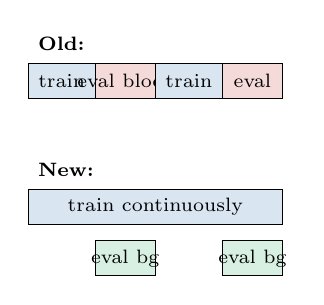
\begin{tikzpicture}[
          every node/.style={font=\scriptsize},
          trainbox/.style={draw,fill=accent!18,minimum width=1.65cm,
                           minimum height=0.48cm,align=center},
          evalbox/.style={draw,fill=green2!18,minimum width=1.35cm,
                          minimum height=0.48cm,align=center},
          deadbox/.style={draw,fill=red2!18,minimum width=1.35cm,
                          minimum height=0.48cm,align=center,text=red2},
          x=0.085cm,
      ]
        \node[font=\scriptsize\bfseries,anchor=west] at (0,2.45) {Old:};
        \draw[trainbox] (0,1.75) rectangle (10,2.2); \node at (5,1.98) {train};
        \draw[deadbox]  (10,1.75) rectangle (19,2.2); \node at (14.5,1.98) {eval block};
        \draw[trainbox] (19,1.75) rectangle (29,2.2); \node at (24,1.98) {train};
        \draw[deadbox]  (29,1.75) rectangle (38,2.2); \node at (33.5,1.98) {eval};

        \node[font=\scriptsize\bfseries,anchor=west] at (0,0.85) {New:};
        \draw[trainbox] (0,0.15) rectangle (38,0.6); \node at (19,0.38) {train continuously};
        \draw[evalbox]  (10,-0.5) rectangle (19,-0.05); \node at (14.5,-0.28) {eval bg};
        \draw[evalbox]  (29,-0.5) rectangle (38,-0.05); \node at (33.5,-0.28) {eval bg};
      \end{tikzpicture}

      \vspace{0.35em}
      \small 44 min of blocked evaluation per 2M-step run eliminated.

    \column{0.50\textwidth}
      \textbf{Throughput}
      \vspace{0.25em}

      \resizebox{\linewidth}{!}{%
      \begin{tabular}{@{}lr@{}}
        \toprule
        Configuration & fps \\
        \midrule
        Run7 full training baseline & \textcolor{red2}{53} \\
        Pre-speedup env-only & 1{,}009 \\
        \textbf{Post-speedup env-only} & \textcolor{green2!70!black}{\textbf{2{,}757}} \\
        \bottomrule
      \end{tabular}}

      \vspace{0.6em}
      \begin{itemize}
        \setlength{\itemsep}{0.35em}
        \item Flat MPD arrays replace list-of-lists hot loops.
        \item Multi-trace precompute cache makes resets cheap.
        \item Numba compiles departure and sticky-load kernels.
      \end{itemize}

      \vspace{0.3em}
      \small\textit{Full-training and env-only fps are labeled separately.}

  \end{columns}

\end{frame}

% =========================================================================
% MAIN SLIDE 9 -- What we learned
% =========================================================================

\begin{frame}[shrink=5]{What the experiments actually say.}

  \begin{columns}[T,onlytextwidth]

    \column{0.33\textwidth}
      \begin{block}{Where RL helps}
        \small
        High-churn workloads where departure timing changes the right MPD choice.
      \end{block}

    \column{0.33\textwidth}
      \begin{block}{Where greedy wins}
        \small
        Long-lived stable load where the least-loaded local MPD is already a
        strong rule.
      \end{block}

    \column{0.33\textwidth}
      \begin{block}{Next bottleneck}
        \small
        Distribution-aware generalization across VM lifetime regimes.
      \end{block}

  \end{columns}

  \vspace{1.0em}
  \begin{itemize}
    \setlength{\itemsep}{0.65em}
    \item RL is not automatically better than greedy; it helps when trace structure
          rewards departure-aware placement.
    \item Reward shaping made the problem measurable, but did not by itself solve
          cross-trace transfer.
    \item The simulator is now fast enough to answer the next questions with
          controlled ablations.
  \end{itemize}

\end{frame}

% =========================================================================
% MAIN SLIDE 10 -- Future work
% =========================================================================

\begin{frame}[shrink=6]{Future work: make the learned policy robust, not just better on one regime.}

  \begin{columns}[T,onlytextwidth]

    \column{0.50\textwidth}
      \begin{itemize}
        \setlength{\itemsep}{0.62em}
        \item Balance training batches by lifetime regime so AMS20-like traces
              are not underrepresented -- figure out non-stationarity.
        \item Does optimal help woth learning?
        \item Expand augmentation only with validated knobs: arrival jitter,
              lifetime perturbation, topology/link failures.
      \end{itemize}

      \vspace{0.3em}
      \small\textit{Deployment framing: keep greedy as a fallback; use RL only
      where departure-aware placement is justified.}

    \column{0.50\textwidth}
      \begin{center}
      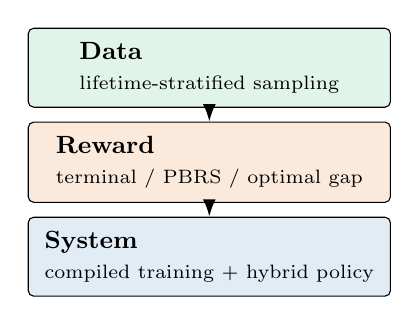
\begin{tikzpicture}[
          every node/.style={font=\small},
          lane/.style={draw,rounded corners=2pt,fill=black!5,
                       minimum width=4.6cm,minimum height=0.78cm,
                       align=left,inner sep=5pt},
          arr/.style={-{Latex[length=2.2mm]},line width=0.8pt},
      ]
        \node[lane,fill=green2!14] (data) at (0,2.6)
          {\textbf{Data}\\\scriptsize lifetime-stratified sampling};
        \node[lane,fill=orange2!16] (reward) at (0,1.4)
          {\textbf{Reward}\\\scriptsize terminal / PBRS / optimal gap};
        \node[lane,fill=accent!14] (system) at (0,0.2)
          {\textbf{System}\\\scriptsize compiled training + hybrid policy};
        \draw[arr] (data) -- (reward);
        \draw[arr] (reward) -- (system);
      \end{tikzpicture}
      \end{center}

  \end{columns}

\end{frame}

% =========================================================================
% BACKUP SLIDES
% =========================================================================

\appendix

\begin{frame}[plain]
  \vfill
  \begin{center}
    {\Large\bfseries Appendix}\\[0.8em]
    \small Extra implementation details and diagnostic backup slides.
  \end{center}
  \vfill
\end{frame}

\begin{frame}[shrink=5]{Backup: what was built.}

  \begin{columns}[T,onlytextwidth]

    \column{0.50\textwidth}
      \begin{block}{Simulator and state}
        \small
        Gymnasium CXL memory-pooling env; online VM-arrival replay; reachable-MPD
        action constraints; departure-aware state with $D_j$, $S_j$, $P_j$, and $Q_j$.
      \end{block}

      \vspace{0.45em}
      \begin{block}{Training data}
        \small
        Ten Azure traces characterized by VM size, arrival rate, lifetime, and pod
        density; 7 train / 1 val / 2 held-out split; episode-level augmentation.
      \end{block}

    \column{0.50\textwidth}
      \begin{block}{RL and reward study}
        \small
        SB3 SAC primary path; LCPO/A2C explored; reward ablation R1--R5 from
        local proxy to terminal/PBRS objective-aligned signals.
      \end{block}

      \vspace{0.45em}
      \begin{block}{Systems engineering}
        \small
        Async eval worker removes blocked callbacks; flat MPD arrays, multi-trace
        cache, and Numba raise env-only throughput to 2{,}757 fps; JAX trainer
        built as compiled alternative.
      \end{block}

  \end{columns}

\end{frame}

\begin{frame}{Backup: Greedy packs load onto a few MPDs; RL spreads it.}

  \begin{columns}[T,onlytextwidth]

    \column{0.50\textwidth}
      \begin{center}
        \textbf{Greedy} \hfill \textcolor{red2}{ratio $\approx$ 6.1}

        \vspace{0.2em}
        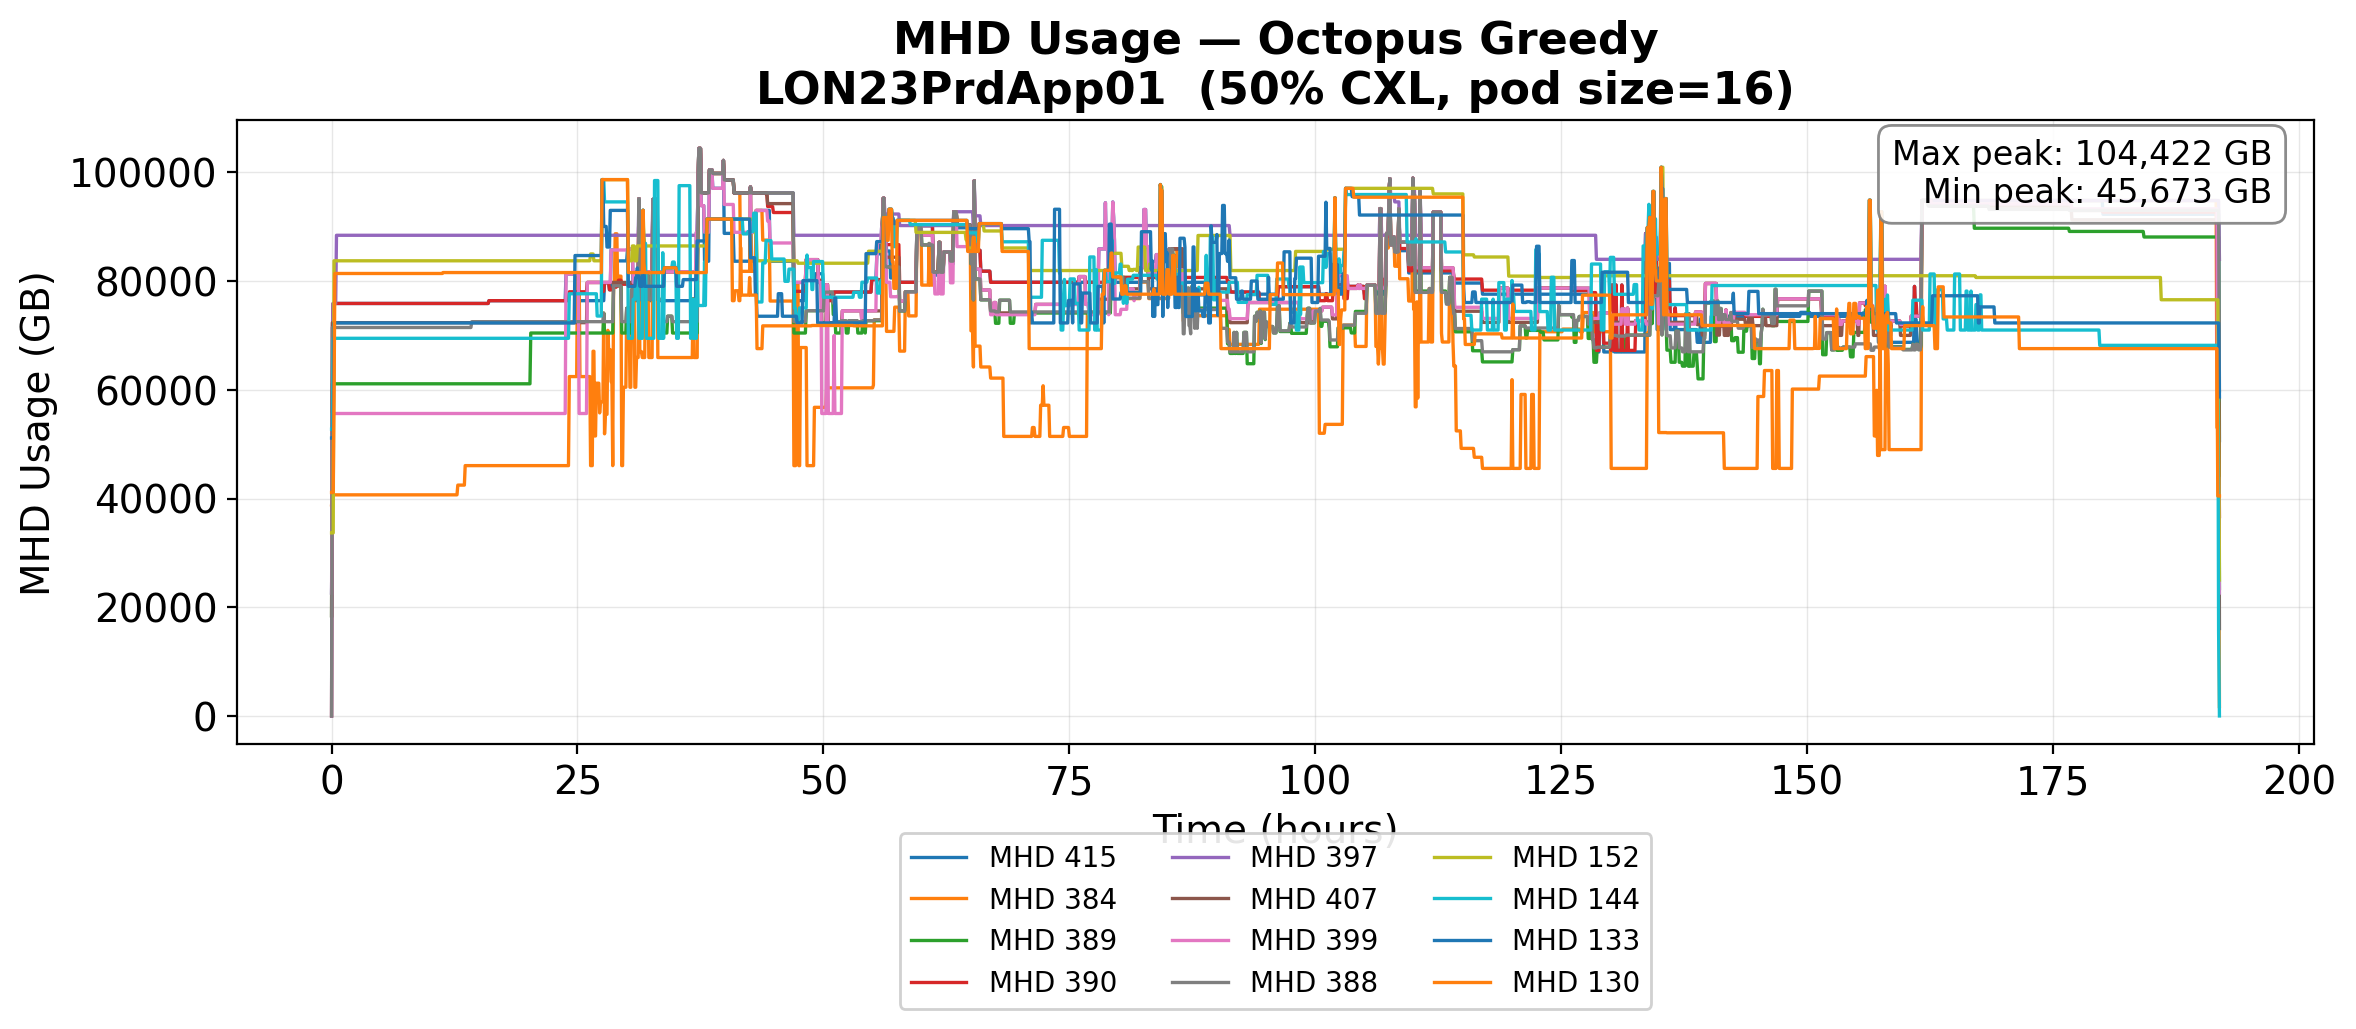
\includegraphics[width=\linewidth]{mhd_timeseries_greedy.png}

        \vspace{0.1em}
        \small A few MPDs saturate; most stay idle.
      \end{center}

    \column{0.50\textwidth}
      \begin{center}
        \textbf{RL (run 7)} \hfill \textcolor{accent}{ratio $\approx$ 1.04}

        \vspace{0.2em}
        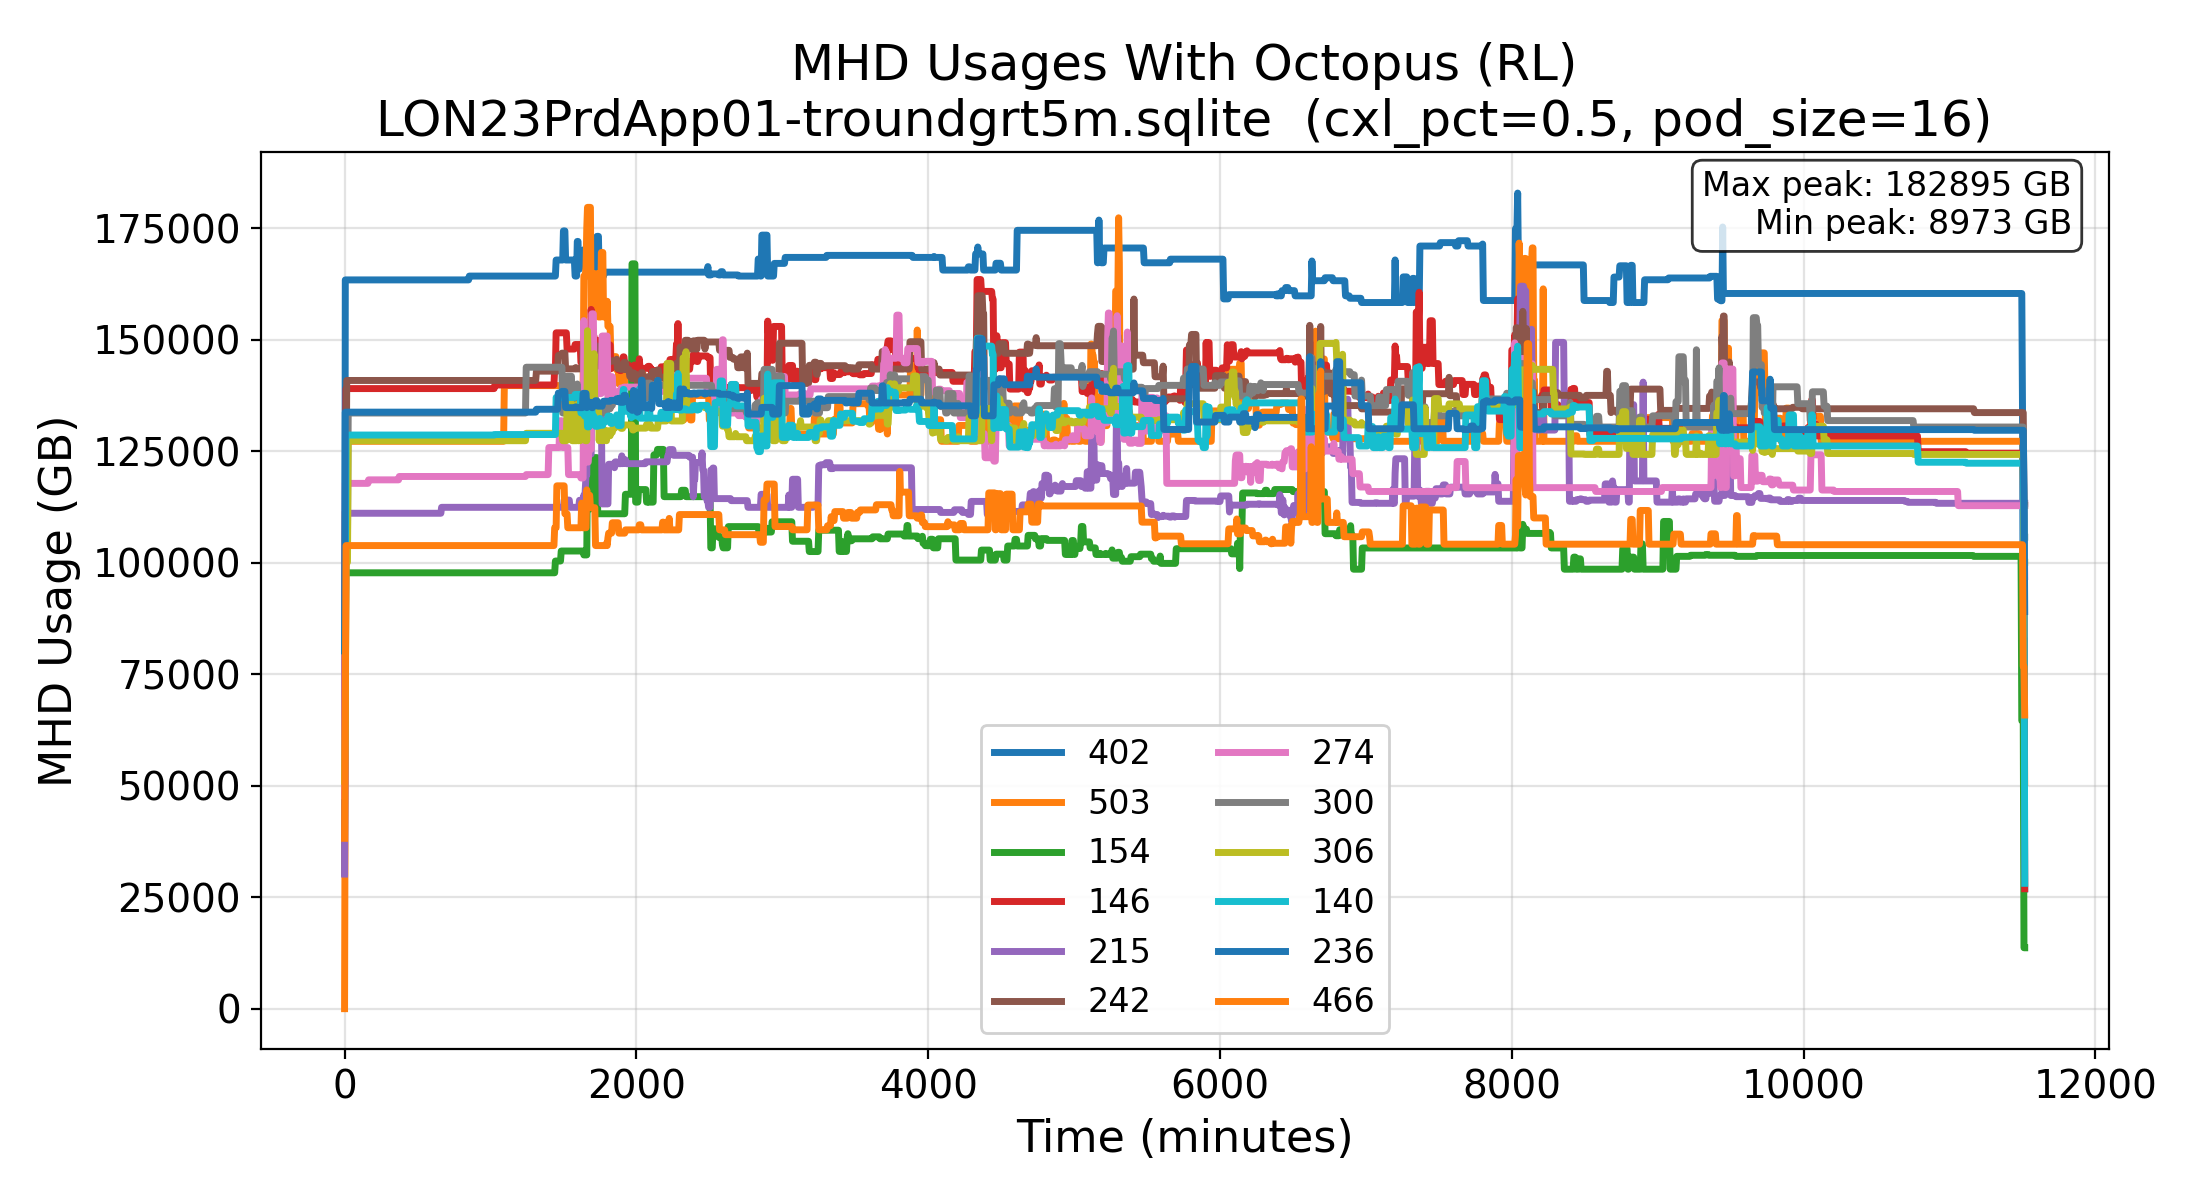
\includegraphics[width=\linewidth]{mhd_timeseries_rl.png}

        \vspace{0.1em}
        \small Load spread across all MPDs; no bottleneck.
      \end{center}

  \end{columns}

  \vspace{0.2em}
  \begin{center}
    \small\textit{LON23 validation trace, CXL fraction 0.5, pod of 16 nodes.
    Each line = one MPD over the replay window.}
  \end{center}

\end{frame}

\begin{frame}[shrink=5]{Backup: SAC objective and why entropy mattered.}

  \begin{columns}[T,onlytextwidth]

    \column{0.48\textwidth}
      \vspace{0.2em}
      \begin{block}{Soft Actor-Critic objective}
        \scriptsize
        \[
          J(\pi)
          =
          \mathbb{E}
          \left[
            \sum_t \gamma^t
            \bigl(r_t + \alpha\,\mathcal{H}(\pi(\cdot \mid s_t))\bigr)
          \right]
        \]
      \end{block}

      \vspace{0.4em}
      \small
      The extra entropy term rewards the policy for keeping probability mass
      across multiple plausible MPDs instead of collapsing immediately to a
      single deterministic placement.

    \column{0.52\textwidth}
      \vspace{0.2em}
      \begin{itemize}
        \setlength{\itemsep}{0.65em}
        \item \textbf{$r_t$:} reward from the placement objective.
        \item \textbf{$\gamma = 0.999$:} long horizon because trace episodes
              have thousands of VM arrivals.
        \item \textbf{$\alpha$:} entropy temperature, auto-tuned by SB3.
        \item \textbf{$\mathcal{H}$:} exploration pressure; low entropy means
              premature collapse.
      \end{itemize}

      \vspace{0.35em}
      \begin{block}{Project-specific reason}
        \small
        Early rewards produced collapsed policies.  SAC made collapse visible
        through \texttt{sac/ent\_coef} and gave the actor pressure to keep exploring.
      \end{block}

  \end{columns}

\end{frame}

\begin{frame}[shrink=6]{Backup: SAC architecture and diagnostics.}

  \begin{columns}[T,onlytextwidth]

    \column{0.60\textwidth}
      \begin{center}
      \resizebox{0.96\linewidth}{!}{%
      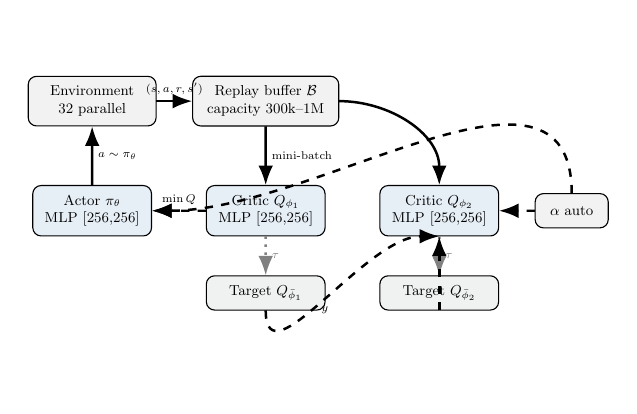
\begin{tikzpicture}[
          scale=0.58,
          transform shape,
          every node/.style={font=\small},
          box/.style={draw,rounded corners=3pt,fill=black!5,
                      minimum height=0.75cm,align=center,inner sep=6pt},
          netbox/.style={draw,rounded corners=3pt,fill=accent!12,
                         minimum height=0.75cm,align=center,inner sep=6pt},
          arr/.style={-{Latex[length=2.5mm]},line width=0.9pt},
          darr/.style={-{Latex[length=2.5mm]},line width=0.9pt,dashed},
          polyak/.style={-{Latex[length=2.5mm]},line width=0.9pt,dotted,gray}
      ]
        \node[box,minimum width=3.2cm] (buf) at (0,0)
          {Replay buffer $\mathcal{B}$\\capacity 300k--1M};
        \node[box,minimum width=2.8cm] (env) at (-3.8,0)
          {Environment\\32 parallel};
        \node[netbox,minimum width=2.6cm] (actor) at (-3.8,-2.4)
          {Actor $\pi_\theta$\\MLP [256,256]};
        \node[netbox,minimum width=2.6cm] (q1) at (0,-2.4)
          {Critic $Q_{\phi_1}$\\MLP [256,256]};
        \node[netbox,minimum width=2.6cm] (q2) at (3.8,-2.4)
          {Critic $Q_{\phi_2}$\\MLP [256,256]};
        \node[box,minimum width=2.6cm,fill=gray2!12] (tq1) at (0,-4.2)
          {Target $Q_{\bar\phi_1}$};
        \node[box,minimum width=2.6cm,fill=gray2!12] (tq2) at (3.8,-4.2)
          {Target $Q_{\bar\phi_2}$};
        \node[box,minimum width=1.6cm] (alpha) at (6.7,-2.4)
          {$\alpha$ auto};

        \draw[arr] (env) -- node[above,font=\scriptsize]{$(s,a,r,s')$} (buf);
        \draw[arr] (actor) -- node[right,font=\scriptsize]{$a \sim \pi_\theta$} (env);
        \draw[arr] (buf) -- node[right,font=\scriptsize]{mini-batch} (q1);
        \draw[arr] (buf.east) to[out=0,in=90] (q2.north);
        \draw[darr] (q1) -- node[above,font=\scriptsize]{$\min Q$} (actor);
        \draw[polyak] (q1) -- node[right,font=\scriptsize]{$\tau$} (tq1);
        \draw[polyak] (q2) -- node[right,font=\scriptsize]{$\tau$} (tq2);
        \draw[darr] (tq1.south) to[out=-90,in=180] node[below,font=\scriptsize]{$y$} (q2.south);
        \draw[darr] (tq2.south) -- (q2.south);
        \draw[darr] (alpha) -- (q2);
        \draw[darr] (alpha.north) to[out=90,in=0] (actor.east);
      \end{tikzpicture}
      }
      \end{center}

      \vspace{0.2em}
      \scriptsize Solid: data flow. Dashed: gradient-coupled terms.
      Dotted: target-network update.

    \column{0.36\textwidth}
      \vspace{0.2em}
      \begin{itemize}
        \setlength{\itemsep}{0.42em}
        \item Replay buffer reuses trace-placement experience.
        \item Twin critics use $\min(Q_1,Q_2)$ to suppress overestimation.
        \item Actor maximizes value while entropy prevents early deterministic collapse.
        \item Auto-$\alpha$ tunes exploration pressure; logged as \texttt{ent\_coef}.
        \item Health checks: critic loss, Q-values, entropy, and pooling savings.
      \end{itemize}

  \end{columns}

\end{frame}

\end{document}
